\chapter{Results}
\label{cha:conclusion}
Each strategy was tested on three realistic temporal network datasets, with its performance measured and plotted. Different runs were made, with increasing budget value and a fixed Pspread as well as runs with fixed budget and increased Pspread. Each of the runs consisted of a sufficiently high number of simulations (average spread was considered as infection value), to get valid results despite the probability factor. The goal of these tests was to develop a 360° view of the strategies under different point of views, and the following aspects are plotted and showed:
\begin{itemize}
    \item Seed Set Size Characterization with budget increment
    \item Performance variation with budget increment
    \item Performance variation with Pspread increment
    \item Performance variation across the different datasets
    \item Performance comparison between strategies
\end{itemize}
The results are displayed according to the dataset and then discussed together in a final report discussion.

\section{College Message Dataset}
\label{sec:collegeres}
This dataset consisted of a total of 1899 nodes and 59835 edges, each one at a different time (so no simultaneous edges), a decent 31 nodes to edges ratio and roughly 1 percent of unreachable nodes.
\begin{center}
    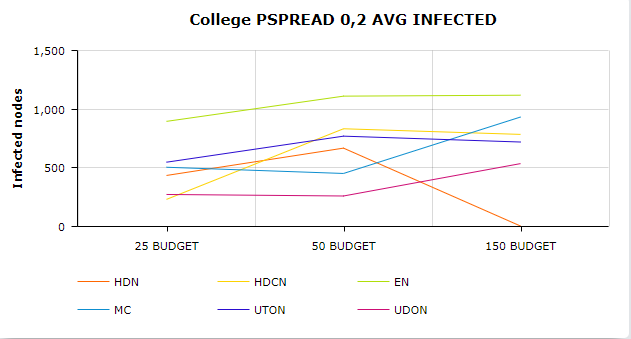
\includegraphics[scale=1]{/resultscollege/college avg performance}
    \\
    Figure 5.1: Overall Performance Of the Strategies on College Dataset
\end{center}

The result shows that the Earliest Nodes strategy was the overall best performing on this dataset(50-60 percent of the nodes). Not only, it was also the only strategy to have a (non-linear) increase of the performance when given more budget, despite the increments not being extremely large.
\begin{center}
    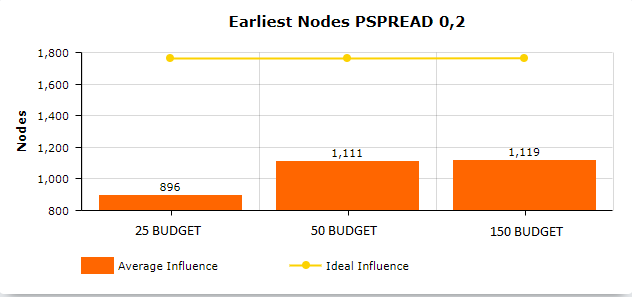
\includegraphics[scale=1]{/resultscollege/earlier performance P02}
    \\
    Figure 5.2: Close Up Performance Of the Earliest Nodes Strategy
\end{center}

This chart shows the progression of the influence with increasing budget, as well as the ideal influence. That is the maximum number of nodes that could have been influenced with this strategy at maximum Probability Pspread = 1. A further run with fixed budget 50 and Pspread = 0.4 was made and it averaged 1417 Infected Nodes (74,6 percent of the nodes). 

\begin{center}
    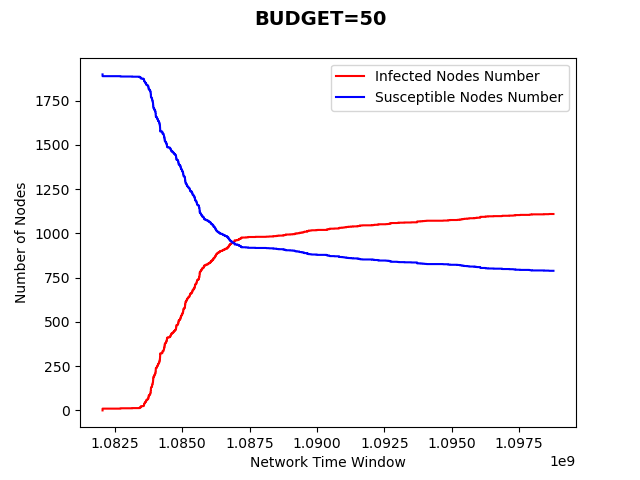
\includegraphics[scale=0.6]{/growth/collegeearlygrowth}
    \\
    Figure 5.3: Curve of Infection for Earliest Nodes PSPREAD 0,2 BUDGET 50
\end{center}
This  chart shows the curve of the infection that the Earliest Nodes Strategy generated with budget 50 and Pspread 0,2. It is easy to see from the chart how the earlier nodes impact the curve; in fact it is growing fast at the beginning and is more linear/stable in the later stages of the simulation. This happens because the seed nodes are highly active in the initial stage of the network, but in the later stages the spreading relies on the actually infected nodes, which are limited to the Pspread value and so the progression is massively slower. What follows is the ideal influence spread growth for the strategy.

\begin{center}
    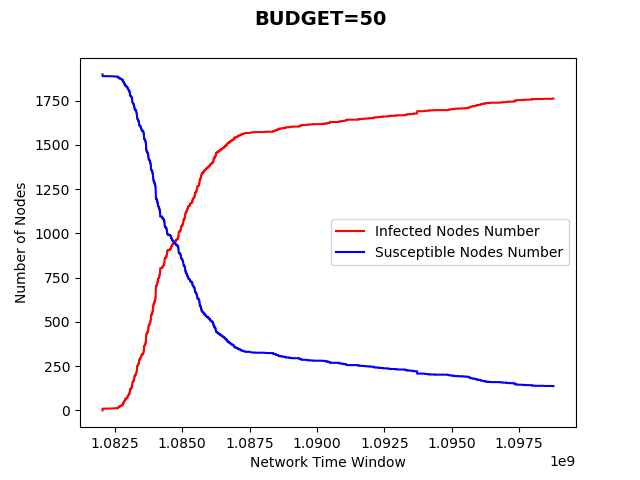
\includegraphics[scale=0.6]{/growth/50-1-college}
    \\
    Figure 5.4: Ideal Curve of Infection for Earliest Nodes PSPREAD 1 BUDGET 50
\end{center}

One noticeable thing is the big downfall of the Highest Degree Nodes Strategy on the test with 150 budget. This is related to one of the main drawbacks of the highest degree strategy: some particular values for the budget can fit exactly one node's cost and therefore the seed set can be small. Moreover, the degree is calculated on the amount of node's messages, meaning that a node with high degree can be also interacting multiple times with the same one node (poor cover). This is something extremely related to the network structure, and as shown in the graph the strategy on 150 budget averaged 4 infected nodes out of 4 maximum infect-able.

\begin{center}
    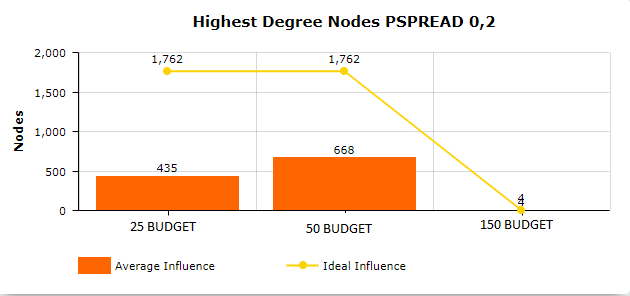
\includegraphics[scale=1]{/resultscollege/greedy performance P02}
    \\
    Figure 5.5: Close Up Performance Of the Highest Degree Nodes Strategy
\end{center}

\begin{center}
    \includegraphics[scale=1]{/resultscollege/seedset}
    \\
    Figure 5.6: Seed Set Size Variation on All Strategies
\end{center}
 The dynamics of the varying node cost also allows seed sets to be not only different in the nodes but also in the overall size. This chart shows that almost every strategy proposed here features an increment of the seed set size with higher budget. This is simply due to the fact that those strategies are not based on picking the highest degree nodes, and more budget allows for more nodes to be seeded, instead of better nodes like in highest degree strategy.

\section{Proximity Conversation Dataset(Ia)}
\label{sec:iares}
This was the strongest connected dataset among all the used ones. It had 20818 edges for only 113 nodes, averaging 184 nodes per edge. Also, only one node in the whole dataset was unreachable or isolated.
\begin{center}
    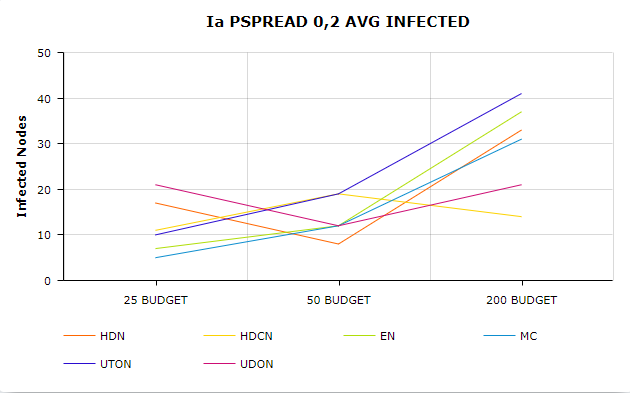
\includegraphics[scale=1]{/resultsia/ia avg performance}
    \\
    Figure 5.7: Overall Performance Of the Strategies on Proximity Dataset Ia
\end{center}

What emerges from the chart is that whatever the budget was, the best strategy was always one of the two that focus on the hardest nodes to reach. That makes sense, because on a strongly connected network like this the majority of the nodes is going to have high in degree, making them getting infected most likely even if they are not seeded or neighbors of the seed nodes. Those strategies allow to include also nodes that are most likely going to be cut out of the network, resulting in an overall better performance as predicted when introducing this network type. \\
However, there were a lot of nodes that were harder to reach than others, and this is shown by the fact that the two strategies based on those nodes had drastically different results at each run. Also, the evolution shows that as the budget increased, the strategies that evolved node degrees were the worst performing, while on lower budget it was the exact opposite.

\begin{center}
    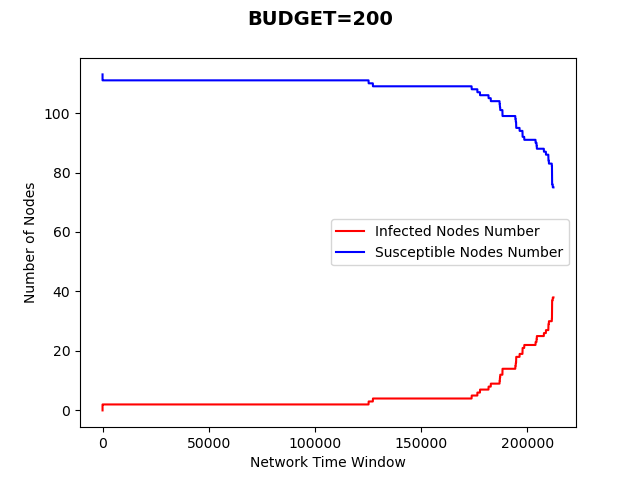
\includegraphics[scale=0.6]{/growth/ia}
    \\
    Figure 5.8: Curve of Infection for Unreachable, Time Oriented Nodes Strategy PSPREAD 0,2 BUDGET 200
\end{center}
The curve clearly reveals some details regarding the structure of the network: the most difficult nodes to reach (the ones with less edges going into them) are all activated in the later to final stages of the network, showing that no relevant Infected - Susceptible interactions occurred during the entire first half of the temporal window, resulting in a potential "waste". However the strategy was still the best on medium-higher budget scenarios.

\begin{center}
    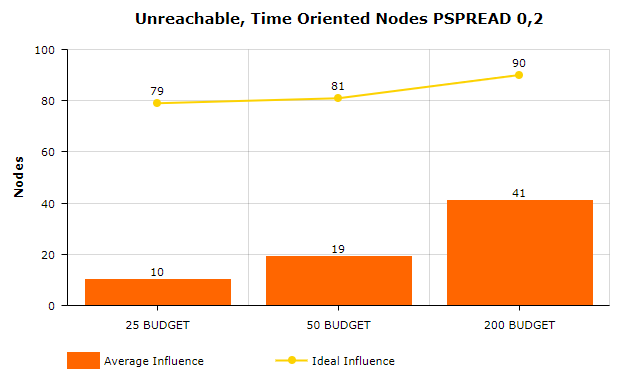
\includegraphics[scale=0.8]{/resultsia/uton performance P02}
    \\
    Figure 5.8: Close Up Performance Of the Unreachable, Time Oriented Nodes Strategy
\end{center}

On this particular dataset the majority of the strategies had a consistent increment of performance with more budget, especially when going from low budgets to a decent budget like 200.

\begin{center}
    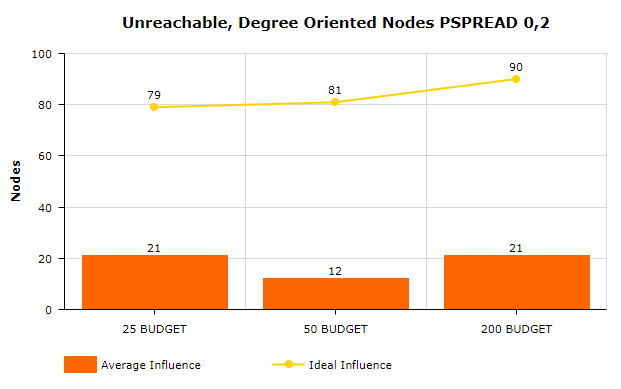
\includegraphics[scale=0.8]{/resultsia/udon preformance P02}
    \\
    Figure 5.9: Close Up Performance Of the Unreachable, Degree Oriented Nodes Strategy
\end{center}

It is interesting to see the big difference between the two Unreachable Nodes oriented strategies. What emerges from the charts is that generally, when the budget is lower the degree of the nodes seems to have more impact in determining the overall performance, whilst with higher budgets the temporal aspect of the networks really make a great difference. On medium-high budget scenarios the worst performing strategy is always some degree related one.

\begin{center}
    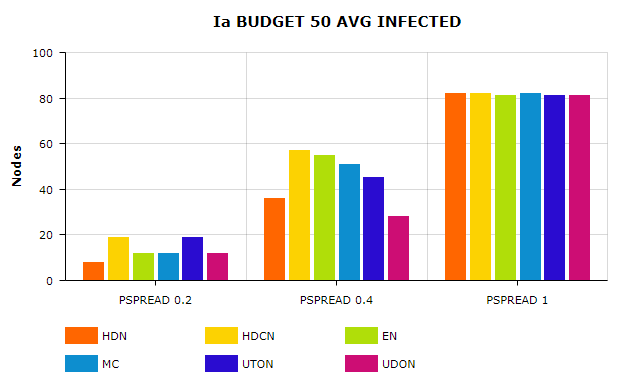
\includegraphics[scale=1]{/resultsia/ia performance prob}
    \\
    Figure 5.10: Performance Variation with increasing Probability
\end{center}

This chart shows that on a highly connected dataset like this one, the overall max performance of each strategy is very similar, however when scaling with the probability spread without saturation there are strategies that get really drastic improvement. These strategies are the ones that either do not consider the quality of the nodes like Maximum Cover Nodes Strategy or the ones that can involve very high-risk high-reward nodes, like the degree based strategies. What generally emerged is that Probability is by far more impactful in a strategy's performance compared to the budget cap.

\section{Chat Dataset(SFHH)}
\label{sec:sfhhres}
This dataset was strongly connected as well, averaging 174 edges per node on a total of 403 nodes. The total number of edges was over 70k, and these were pretty homogeneously distributed between the nodes, as the maximum reach of ideal infection was nearly the same for all the strategies on each run. This made the seed choice even more impactful for the spreading performance. Finally, this network had only 5 unreachable nodes.
\begin{center}
    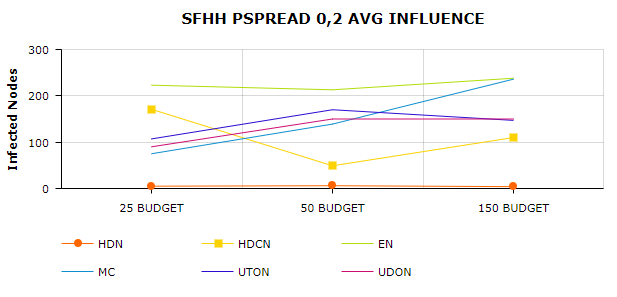
\includegraphics[scale=1]{/resultssfhh/avgperformance}
    \\
    Figure 5.11: Overall Performance Of the Strategies on Chat Dataset SFHH
\end{center}

As the chart shows, the Earlier Nodes strategy was consistently the best, with only the Maximum Cover strategy coming close to it on the higher budget run, but still not topping it. Degree based strategies proved to be generally the worst, with generic highest degree strategy showing an awful performance, while both Unreachable Node based Strategies were solid third and fourth place in every run. It is also noticeable how their values are closer than in every other dataset, and that is because with this particular network structure the unreachable nodes were exclusive, which means there were no nodes with equal low in-degree which is what leads to the strategies always seeding the same nodes. The slight gap in the performance is given by the fact that the average Infection is calculated on a finite number of runs, and it can be a little bit off but not enough to compromise the results. 


\begin{center}
    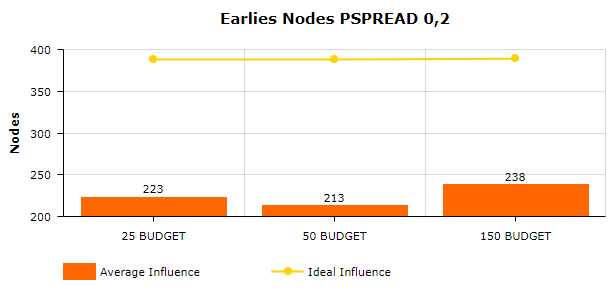
\includegraphics[scale=1]{/resultssfhh/early performance}
    \\
    Figure 5.12: Close Up Performance Of the Earlier Nodes Strategy
\end{center}

An interesting thing here is that despite being the best among the strategies on each single run, averaging 56 percent of total nodes infected, this strategy did not show any important performance boost when fed with more budget. We have learned from previous data sets that budget cap can be tricky, because it can allow higher degree nodes to be seeded that might can have less impact than expected on the influence spread.
\\
Also, being a strongly connected network made every strategy have similar ideal influence results (roughly 95-96 percent of the total nodes, however only EN averaged more than 50 percent of actually influenced nodes on each run, meaning that a correct seed set choice was very crucial. 
\\
\\
Another interesting observation is the curve of infection generated by this strategy, which merges the spreading of the best strategies on the other datasets: in fact, here the curve presents a fast growth in the initial stages of the network, as the strategy is supposed to, followed by a stalling phase in the entire mid range of the network and a final growth again in the later stages.

\begin{center}
    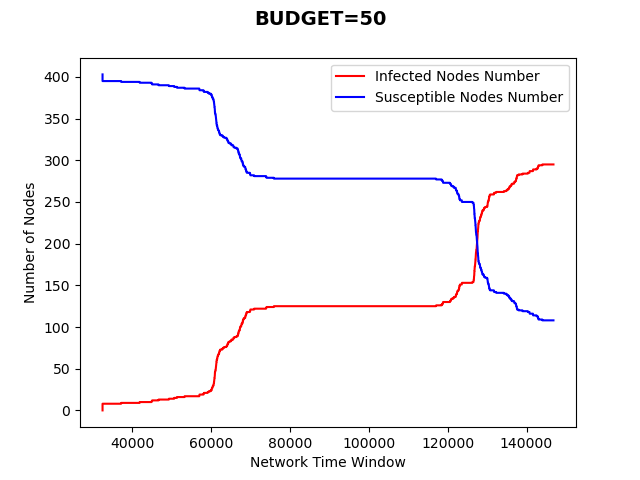
\includegraphics[scale=0.8]{/growth/testgrowth}
    \\
    Figure 5.13: Curve Of Infection for the Earlier Nodes Strategy
\end{center}

The seed set size behaviour was also really interesting: in this dataset the seed sets were generically small on the highest budget run, as going from 50 to 150 budget characterized a drop in the seed set cardinality from values around 8 to seed sets of 1 or 2 nodes, except for two strategies who had pretty consistent seed set size. This enabled nodes of cost just slightly under the budget cap to be seeded, dropping the cardinality by a lot; noticeable is how this did not happen in EN and MC, giving us further information on the network structure. Earlier nodes were generally cheaper, and the cascades generated by them were the ones maximizing the nodes cover, although the seed sets of the two strategies was different by just one node.
This allows us to claim that this network was strongly time dependent, meaning that the earlier nodes were the best both for covering the network but also for actually maximizing the spread of influence.

\begin{center}
    \includegraphics[scale=0.8]{/resultssfhh/seedset}
    \\
    Figure 5.14: Seed Set Size Variation with increasing Budget
\end{center}